\chapter{HLASM overview}

Ordinary assembly languages consist solely of ordinary machine instructions. High-level assemblers generally extend them with features commonly found in high-level programming languages, such as control statements similar to \emph{if, while, for} as well as custom callable macros.

IBM High Level Assembler (HLASM) satisfies this definition and adds other features which will be described in this section.

\section{Syntax}

HLASM syntax is similar to a common assembler, but due to historical reasons it has limitations, like line length limited to 80 characters (as that was the length of a punched card line).

\subsection{Statement}

HLASM program consists of a sequence of \emph{statements}. A statement consists of four fields separated by spaces that can be split into more lines using continuations (see \cref{Continuation}). They are used to produce both compile-time code and run-time code (see \cref{Assembling}). The fields are:
\begin{itemize}
	\item \textbf{Name field} --- Serves as a place for named constants that are to be used in the code. This field is optional, but, when present, it must start at the begin column of a line.
	
	\item \textbf{Instruction field} --- The only mandatory field represents the instruction that is executed. It must not begin in the first column, as it would be interpreted as a name field.
	
	\item \textbf{Operands field} --- Field for instruction operands, located immediately after instruction field. Individual operands must be separated by a comma, and, depending on the specific instruction, can be either blank, in a form of an apostrophe separated string, or represented by a sequence of characters.
	
	\item \textbf{Remark field} --- Optional, serves as inline commentary. Located either after the operands field, or, in case the operands are omitted, after the instruction field. 
\end{itemize}

\begin{listing}[t]
	\begin{verbatim}
name    instruction     operands             remark
.NOMOV       AGO     (&WH).L1,.L2,.L3     SEQUENTIAL BRANCH
	\end{verbatim}
	\caption{An example statement.}
	\label{lst:small_example}
\end{listing}

\Cref{lst:small_example} shows an example of a basic statement containing all fields.

\subsection{Continuations}
\label{Continuation}

Individual statements sometimes contain more than 80 characters, which does not fit to the historic line length limitations. Therefore, a special feature called \emph{continuation} was introduced.

For this purpose the language specification defines four special columns:
\begin{itemize}
	\item \emph{Begin column} (default position: 1)
	
	\item \emph{End column} (default position: 71)
	
	\item \emph{Continuation column} (default position: 72)
	
	\item \emph{Continue column} (default position: 16)
\end{itemize}

The begin column defines where the statements can be started.

The end column determines the position of the end of the line. Anything written to the right of it  does not count as content of the statement, and is rather used as a line sequence number (see \cref{fig01:line}).

The continuation column is used to indicate that the statement continues on the next line. For proper indication, an arbitrary character other than space must be written in this column. The remainder of the statement must then start on the continue column.

An example of an instruction where its last operand exceeded column 72 of the line can be seen in \cref{lst:overflow}.

\begin{listing}[t]
	\begin{verbatim}
    OP1                            REG12,REG07,REG04,REG00,REG01,REG11,Rx
                EG02
	\end{verbatim}
	\caption{Example program that uses the continuation for overflowing the line.}
	\label{lst:overflow}
\end{listing}

Some instructions also support the \emph{extended format} of the operands. That allows the presence of a continuation character even when the contents of a line have not reached the continuation column (see \cref{lst:extended}).

\begin{listing}[t]
	\begin{verbatim}
          AIF   ('&VAR' FIND '~').A,     REMARK1                        x
                ('&VAR'  EQ  'L').B,     REMARK2                        x
                (T'&VAR  EQ  'U').C      REMARK3 
	\end{verbatim}
	\caption{Extended instruction format.}
	\label{lst:extended}
\end{listing}

\begin{figure}
	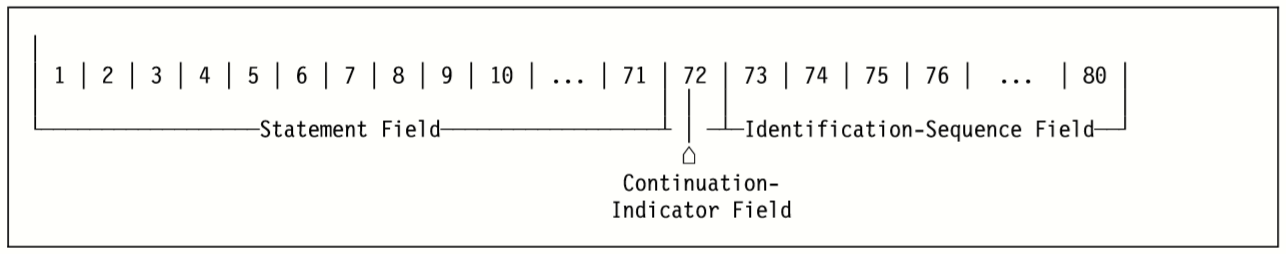
\includegraphics[width=\textwidth]{img/line}
	\caption{Description of line columns (source: \href{https://www-01.ibm.com/servers/resourcelink/svc00100.nsf/pages/zOSV2R3sc264940/$file/asmr1023.pdf}{HLASM Language Reference} ).}
	\label{fig01:line}
\end{figure}


\section{Assembling}
\label{Assembling}

Having briefly described the syntax, now we describe the assembly process hidden behind HLASM. 

We distinguish two types of processing: \emph{Conditional Assembly (CA) processing} and \emph{Ordinary processing}.

The ordinary processing works with \emph{machine instructions} and \emph{assembler instructions} (see \cref{mach_instr}, \cref{asm_instrs}). The main purpose of CA processing (see \cref{CA_proc}) is to generate statements for ordinary assembly.

\subsection{Ordinary assembly}

With help of machine and assembler instructions, the ordinary assembly processing is responsible for runtime behaviour of the program. Ordinary assembly allows to produce code from traditional machine instructions, special-purpose assembler instructions and save values in \emph{ordinary symbols}.

\subsubsection{Ordinary symbols}

In HLASM, an \emph{ordinary symbol} is a named constant that can represent either a simple integer or an address. It can be defined by writing its name into the name field of a statement. Each ordinary symbol can only be defined once, and its value is constant. There are two kinds of ordinary symbols:
\begin{itemize}
	\item An \emph{absolute symbol} that simply has an integral value. It can be defined using a special assembler instruction.
	\item A \emph{relocatable symbol} that represents an address in the resulting object code. It can be defined by writing the ordinary symbol name into the name field of a statement with a machine instruction and denotes the address of the instruction.
\end{itemize}

\subsubsection{Machine instructions}
\label{mach_instr}

\emph{Machine instructions} represent the actual processor instructions executed during run-time. The assembler translates them into corresponding opcodes and processes their operands. That does not differ from traditional assemblers. In contrast to that, HLASM allows expressions to be passed as operands of the instructions. These expressions may use ordinary symbols and support integer and address arithmetic.

\subsubsection{Assembler instructions}
\label{asm_instrs}

In addition to machine instructions, the HLASM assembler provides the \emph{assembler instructions} (in other systems commonly termed as \emph{directives}). They instruct the assembler to make specific actions rather than to assemble opcodes. For example, they generate run-time data constants, create ordinary symbols, organize the resulting object code and generally affect how the assembler operates.

The assembler instructions include the following examples:
\begin{itemize}
	\item \textbf{ICTL} --- Changes values of the previously described line columns (i.e. begin column may begin at column 2 etc.).
	
	\item \textbf{DC}, \textbf{DS} --- Reserves space in object code for data described in operands field and assembles them in place (i.e. assembles float, double, character array, address etc.).
	
	\item \textbf{EQU} --- Defines ordinary symbols.
	
	\item \textbf{COPY} --- Copies text from a specified file\footnote{Path to the folder of the file is passed to assembler before the start of assembly} and pastes it in place of the instruction. It is very similar to the C preprocessor \texttt{\#include} directive.
	
	\item \textbf{CSECT} --- Creates an executable control section. Serves as the beginning of a machine instruction sequence and as the start of relative addressing.
\end{itemize}

\subsubsection{Ordinary symbols resolution}
\label{ordinary_resolution}
All the assembler instructions and ordinary symbols must be resolved before the assembler writes the final object file. The HLASM language supports forward declaration of ordinary symbols, so the assembly may be quite complicated. Consider an example in \cref{lst:ordinary_assembly}. When the instruction in line 1 is seen for the first time, it is impossible to determine its length, because the symbol \verb|LEN| is not defined yet \footnote{Character L with an expression in parentheses in DS operand of type C specifies how many bytes should be reserved in the program.}. The same applies to the length of the instruction in the second line. Furthermore, it is also impossible to determine the exact value of relocatable symbols \verb|ADDR| and \verb|HERE|, because of the unknown length of the preceding instructions.

\begin{listing}[t]
	\begin{verbatim}
	
	[01]              DS    CL(LEN)
	[02]   ADDR       DS    CL(SIZE)
	[03]
	[04]   HERE       DS    0H
	[05]   LEN        EQU   HERE-ADDR
	[06]   SIZE       EQU   1
	
	\end{verbatim}
	\caption{A sample program that shows that symbols can be used prior to their definition.}
	\label{lst:ordinary_assembly}
\end{listing}


In the next step, \verb|LEN| is defined, but it cannot be evaluated, because the subtraction of addresses \verb|ADDR| and \verb|HERE| is dependent on the unknown length of instruction on second line and therefore on the symbol \verb|SIZE|. The whole program is resolved only when the assembly reaches the last line, which defines the length of instruction \verb|02|. Afterwards, it is possible to resolve \verb|LEN| and finally the length of instruction \verb|01|.

The dependency graph created by these principles can be arbitrarily deep and complicated, however it must not contain cycles (a symbol must not be transitively dependent on itself).

\subsection{Conditional assembly}
\label{CA_proc}

On top of machine and assembler instructions, the HLASM assembler offers the conditional assembly. The user may think of it as a macro-language built above traditional assembler. It alters textual representation of the source code and selects which lines will be processed next. Conditional assembly instructions may define \emph{variable symbols} which can be used in any statement to alter its meaning. Moreover, it is possible to define \emph{macros} --- reusable pieces of code with parameters.

\subsubsection{Variable symbols}

Variable symbols serve as points of substitution or information holders. 

When they occur in a statement, they are substituted by their value to create a statement processable by ordinary assembly. For example, in this manner, a user can write a variable symbol in an operation field of a statement and generate any instruction that can be a result of a substitution.

Variable symbols also have notion of their type --- they can be defined either as an integer, a boolean or a string. CA instructions gather this information for different sorts of conditional branching.

\subsubsection{CA instructions}

CA instructions are not assembled into object code. Rather, they select which instructions will be processed by assembler next.

There are instructions capable of conditional and unconditional branching. HLASM provides a variety of built-in binary or unary operations on variable symbols, which can create complex conditional expressions. This is important in HLASM, as the user can alter flow of instructions that will be assembled into executable program.

Another subset of CA instructions operates on variable symbols. With them, the user can define variable symbols locally or globally, assign or update their values.

\subsubsection{Macros}

A \emph{macro} is a structure consisting of a \emph{name}, \emph{input parameters} and a \emph{body}, which is a sequence of statements. When a macro is called in a HLASM program, each statement in its body is executed. Both nested and recursive calls of macros are allowed. Macro body can contain CA instructions or even a sequence of instructions generating another macro definition. With the help of variable symbols, HLASM macros have the power to create custom, task specific macros.

\vspace{5mm}

An example of simple HLASM program with the description of its statements is shown in \cref{lst:example}.

In lines \verb|01-04|, we see a \emph{macro definition}. It is defined with a name \verb|GEN_LABEL|, variable \verb|NAME| and contains one instruction in its body, which assigns the current address to the label in \verb|NAME|.

In line \verb|06|, the \emph{copy instruction} is used, which includes the contents of the \verb|REGS| file.

Line \verb|08| establishes a start of an executable section \verb|TEST|. 

In line \verb|09|, an integer value is assigned to a variable symbol \verb|VAR|. The value is the length attribute of previously non-defined constant \verb|DOUBLE|. The assembler looks for the definition of the constant to properly evaluate the conditional assembly expression. In the next line, there is CA branching instruction \verb|AIF|. If value of \verb|VAR| equals to 4, next lines are skipped and assembling continues on line \verb|18|, where branching symbol \verb|.END| is located. In that case, all the text between the \verb|AIF| and \verb|.END| is completely skipped --- it does not even have to be valid HLASM code.

Lines \verb|12-13| show examples of machine instructions that are directly assembled into object code. Lines \verb|11| and \verb|14| contain examples of macro call.

In line \verb|15|, the constant \verb|LEN| is assigned the difference of two addresses, which results in absolute ordinary symbol. This value is next used to generate character data.

Instruction \verb|DC| in line \verb|17| creates value of type double and assigns its address to ordinary symbol \verb|DOUBLE|. This constant also holds information about length, type and other attributes of the data.  

\verb|ANOP| is an empty assembler action which defines the \verb|.END| symbol and line \verb|19| ends the assembling of the program. 

\begin{listing}[t]
	\begin{verbatim}
	name        operation   operands
	
	[01]                 MACRO                   
	[02]     &NAME       GEN_LABEL
	[03]     &NAME       EQU         *
	[04]                 MEND
	[05]             
	[06]                 COPY        REGS
	[07]             
	[08]     TEST        CSECT
	[09]     &VAR        SETA        L'DOUBLE
	[10]                 AIF         (&VAR EQ 4).END
	[11]     LBL1        GEN_LABEL
	[12]                 LR          3,2
	[13]                 L           8
	[14]     LBL2        GEN_LABEL
	[15]     LEN         EQU         LBL2-LBL1
	[16]                 DC          (LEN)C'HELLO'
	[17]     DOUBLE      DC          H'-3.729'
	[18]     .END        ANOP
	[19]                 END
	\end{verbatim} 
	\caption{An example of an artificial HLASM program.}
	\label{lst:example}
\end{listing}

\vspace{5mm}

Although CA processing may act like a text preprocessing, it is still interlinked with ordinary processing. CA has mechanics that allows the assembler to gather information about statements that are printed during the processing. It can access values created in ordinary assembly and use them in conditional branching. CA is able to lookup constants that are not yet defined prior to the currently processed statement. Moreover, during ordinary assembly, names of these instructions can be aliased.

To sum up, CA processing has variables to store state of compilation and CA instructions for conditional branching. Hence, it is Turing-complete while still evaluated during compile-time.


